\documentclass[11pt]{article}

\usepackage{amssymb}
\usepackage{amsthm}
\usepackage{amsmath}
\usepackage[table]{xcolor}
\usepackage{enumitem}
\usepackage{multirow}
\usepackage{hyperref}
\usepackage{graphicx}
\usepackage{cleveref}
\hypersetup{
  colorlinks, urlcolor = blue
}

\usepackage{array}
\newcolumntype{L}[1]{>{\raggedright\let\newline\\\arraybackslash\hspace{0pt}}m{#1}}
\newcolumntype{C}[1]{>{\centering\let\newline\\\arraybackslash\hspace{0pt}}m{#1}}
\newcolumntype{R}[1]{>{\raggedleft\let\newline\\\arraybackslash\hspace{0pt}}m{#1}}


\begin{document}

\title{\endgraf\rule{\textwidth}{.4pt}\\Model-Agnostic Meta-Learning (MAML) - No 2(b)}
\author{David Ishak Kosasih (20195033)}
\date{\today\endgraf\rule{\textwidth}{.4pt}}
\maketitle

%%%%%%%%%%%%%%%%%%%%%%%%%%%%%%%%%%%%%%%%%%%%%%%%%%%%%%%%%%%%%%%%%%%%
% explenation	

For this experiment, I decreased the number of task for the task distribution to 50000 in order to reduce memory consumption. Moreover, I also fixed the maximum number of epoch to 30000; however, for some experiments I stopped the training process when the network started to converge. 

\begin{figure}[ht]
	\centering
	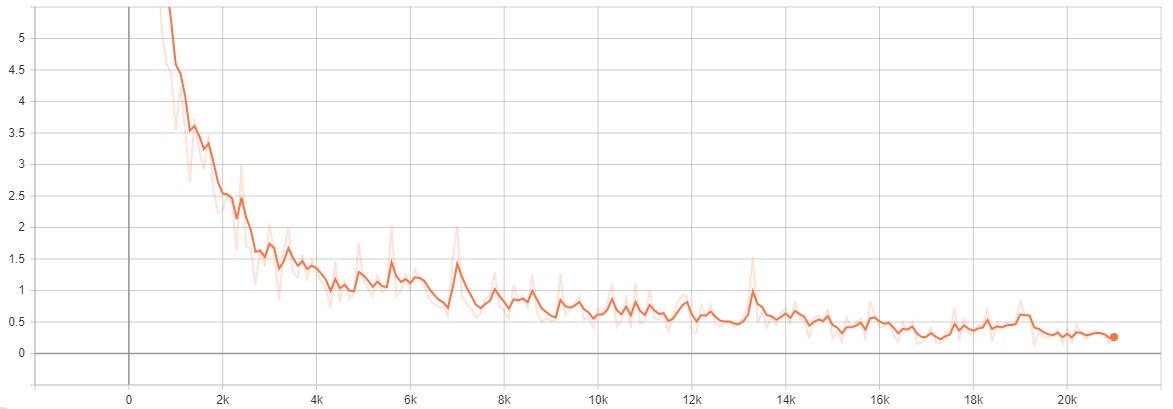
\includegraphics[width=0.7\linewidth]{Images/omninglot 5 way - 1 shot alpha = 0.4}
	\caption{Meta-validation loss for omniglot 5 way 1 shot, alpha = 0.4}
	\label{fig:o5w1sa0.4}
\end{figure}

\begin{figure}[ht]
	\centering
	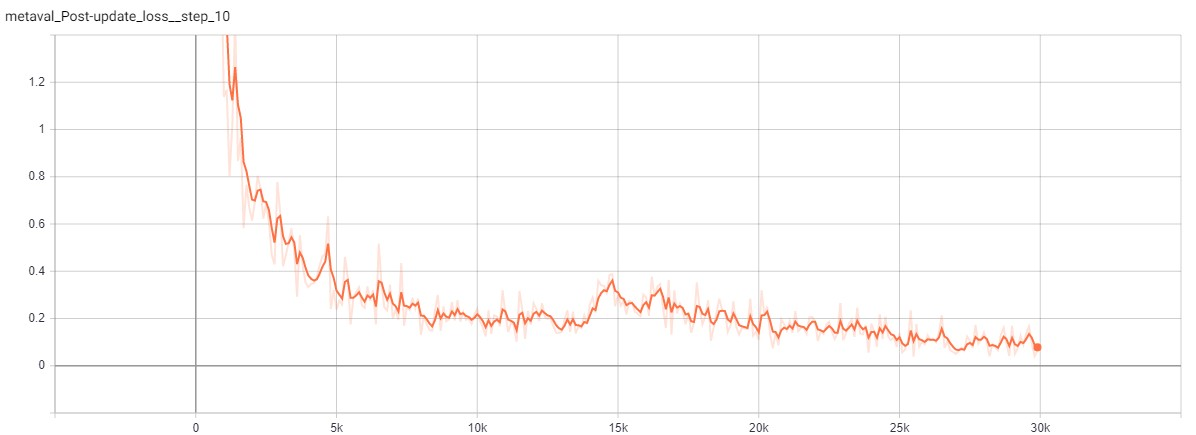
\includegraphics[width=0.7\linewidth]{Images/omniglot 5 way - 5 shot alpha = 0.4}
	\caption{Meta-validation loss for omniglot 5 way 5 shot, alpha = 0.4}
	\label{fig:o5w5sa0.4}
\end{figure}

\begin{figure}[ht]
	\centering
	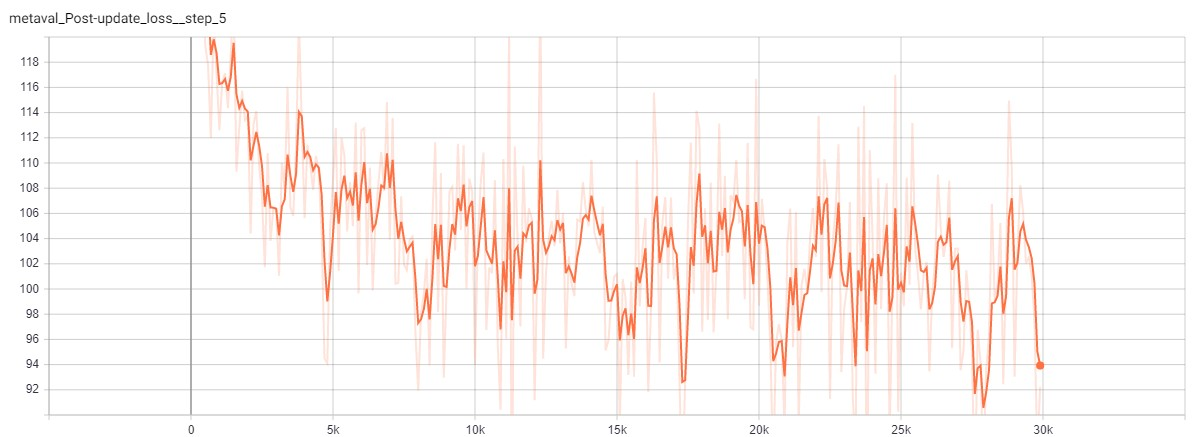
\includegraphics[width=0.7\linewidth]{Images/miniimagenet 5 way - 1 shot}
	\caption{Meta-validation loss for \emph{mini}Imagenet 5 way 1 shot alpha = 0.01}
	\label{fig:m5w1s}
\end{figure}

\begin{figure}[ht]
	\centering
	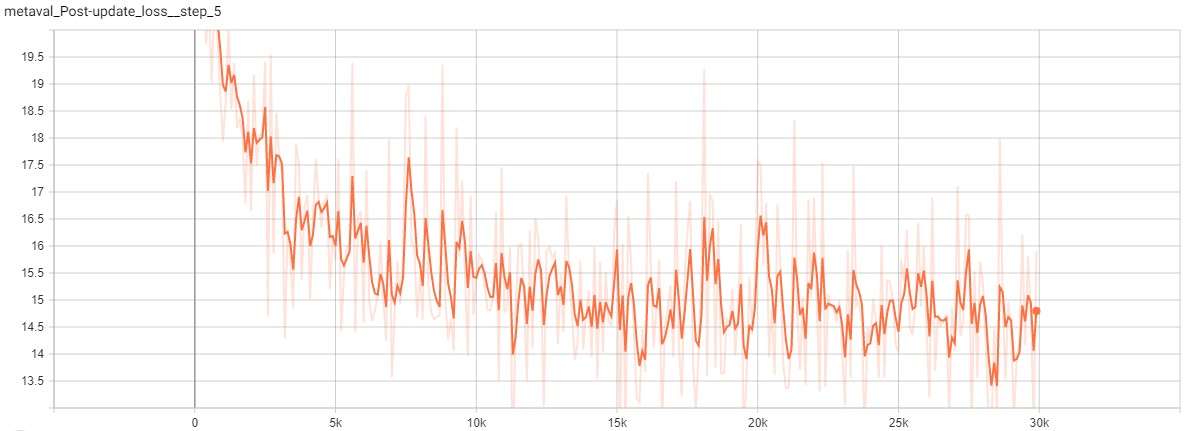
\includegraphics[width=0.7\linewidth]{Images/miniimagenet 5 way - 5 shot}
	\caption{Meta-validation loss for \emph{mini}Imagenet 5 way 5 shot alpha = 0.01}
	\label{fig:m5w5s}
\end{figure}

\Cref{fig:o5w1sa0.4,fig:o5w5sa0.4,fig:m5w1s,fig:m5w5s} showed that the model converge more quickly when it's evaluated on omniglot dataset compared to when it's evaluated on \emph{mini}Imagenet dataset. For omniglot dataset, it started to converge only after approximately 5000 epoch. On the other hand, when \emph{mini}Imagenet was used to evaluate the model, it didn't start to converge even after 30000 epoch. In my opinion, there are at least two things that contributed to this result :

\begin{enumerate}[topsep=0pt,itemsep=-1ex,partopsep=1ex,parsep=1ex]
	\item Different learning rate.
	\begin{description}[style=unboxed,leftmargin=0.2cm]
		\item In this experiment, I fixed the learning rate to 0.4 and 0.01 for omniglot and \emph{mini}Imagenet dataset respectively.
	\end{description}
	\item Dataset
	\begin{description}[style=unboxed,leftmargin=0.2cm]
		\item As we already know, \emph{mini}Imagenet dataset is more challenging or complicated that omniglot dataset.
	\end{description}
\end{enumerate} 

\begin{figure}[ht]
	\centering
	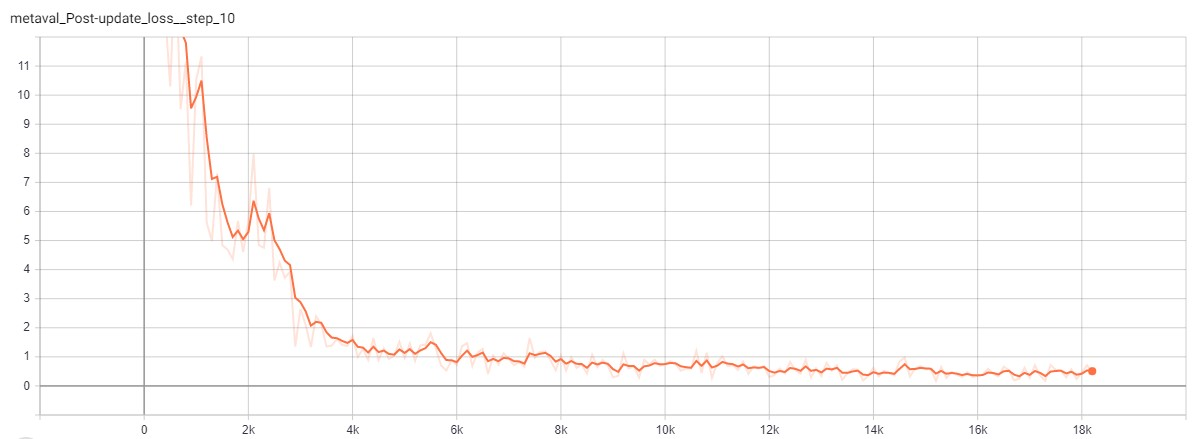
\includegraphics[width=0.7\linewidth]{Images/omninglot 5 way - 1 shot alpha = 1}
	\caption{Meta-validation loss for omniglot 5 way 1 shot, alpha = 1}
	\label{fig:o5w1sa1}
\end{figure}

\begin{figure}[ht]
	\centering
	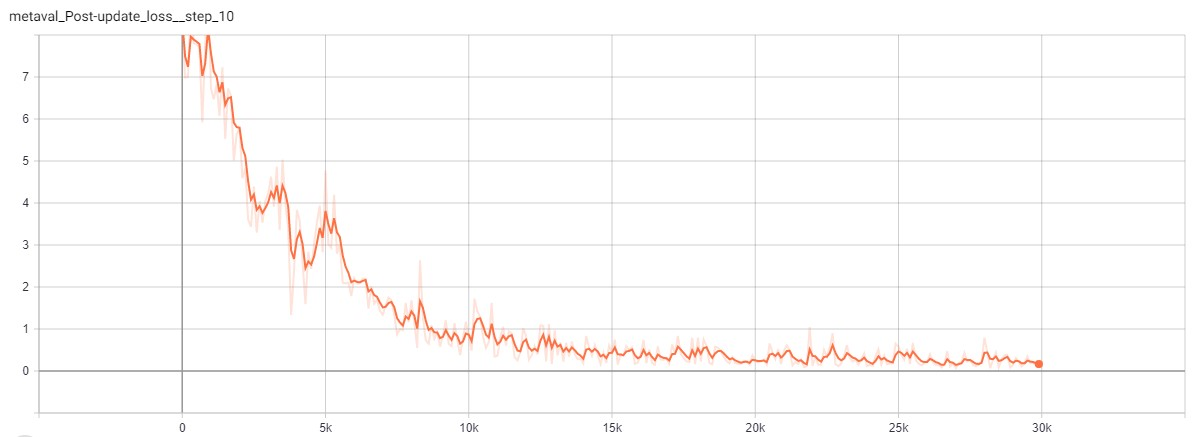
\includegraphics[width=0.7\linewidth]{Images/omniglot 5 way - 5 shot alpha = 1}
	\caption{Meta-validation loss for omniglot 5 way 5 shot, alpha = 1}
	\label{fig:o5w5sa1}
\end{figure}

According to the theory, when we increase the learning rate, our model should learn more quickly. The prove of this hypothesis can be seen in \cref{fig:o5w1sa1,fig:o5w5sa1} as the model took less time to converge when the learning rate was fixed to 1. As for the accuracy, it also yielded better result in this experiment. The drawback of this approach is that our model may never converge if we set the learning rate too big since it can end up jumping randomly; however, since I fixed the learning epoch to a relatively small value for this kind of task, this problem didn't happen.   
	

\end{document}